\documentclass{article}
\usepackage{amsmath,amssymb,graphicx,caption}
\usepackage[utf8]{inputenc}
\usepackage{hyperref}

\title{Thermodynamic Diffusion: A Minimal DDPM Implementation}
\author{}
\date{}

\begin{document}

\maketitle

\section{Introduction}

This artifact demonstrates a minimal Denoising Diffusion Probabilistic Model (DDPM) on MNIST, foregrounding the thermodynamic origins of diffusion models. The forward diffusion process is \textbf{thermodynamic relaxation}: structured signal dissipating toward maximum entropy (isotropic Gaussian noise). The reverse process is \textbf{learned energy-gradient descent}: a neural network recovering structure from noise by estimating the score function.

\section{Mathematical Substrate}

\subsection{Forward Process (Dissipation)}

A Markov chain incrementally adds Gaussian noise:
\begin{equation}
q(x_t | x_{t-1}) = \mathcal{N}(x_t; \sqrt{1 - \beta_t} \cdot x_{t-1}, \beta_t \cdot \mathbf{I})
\end{equation}

With closed-form marginal:
\begin{equation}
q(x_t | x_0) = \mathcal{N}(x_t; \sqrt{\bar{\alpha}_t} \cdot x_0, (1 - \bar{\alpha}_t) \cdot \mathbf{I})
\end{equation}

where $\alpha_t = 1 - \beta_t$ and $\bar{\alpha}_t = \prod_{s=1}^{t} \alpha_s$.

\textbf{Thermodynamic reading:} $\bar{\alpha}_t$ is the \textit{remaining signal fraction} at timestep $t$. As $t \to T$, $\bar{\alpha}_t \to 0$, and $x_t \to \mathcal{N}(0, \mathbf{I})$ --- thermodynamic equilibrium.

\subsection{Reverse Process (Formation)}

The learned reverse:
\begin{equation}
p_\theta(x_{t-1} | x_t) = \mathcal{N}(x_{t-1}; \mu_\theta(x_t, t), \sigma_t^2 \cdot \mathbf{I})
\end{equation}

where $\mu_\theta$ is parameterised via noise prediction $\epsilon_\theta(x_t, t)$, which approximates the \textbf{score function} $\nabla_x \log p(x_t)$.

\subsection{Training Objective}

\begin{equation}
\mathcal{L}_{\text{simple}} = \mathbb{E}_{t, x_0, \epsilon} \left[ \| \epsilon - \epsilon_\theta(x_t, t) \|^2 \right]
\end{equation}

\textbf{Thermodynamic reading:} We train the network to learn the \textbf{exact entropy gradient} at every point along the dissipation trajectory.

\section{Implementation}

\subsection{Architecture}

\begin{itemize}
    \item \textbf{Constraint Field:} U-Net with time-step modulation (sinusoidal embedding)
    \item \textbf{Dissipation Schedule:} Linear $\beta_t \in [0.0001, 0.02]$ over $T=1000$ steps
    \item \textbf{Substrate:} MNIST (28$\times$28 grayscale, normalised to $[-1, 1]$)
    \item \textbf{Training:} Adam ($\text{lr}=2\text{e-}4$), batch size 128, EMA decay 0.9999
\end{itemize}

\subsection{Results}

\begin{figure}[h]
    \centering
    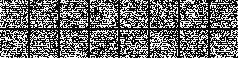
\includegraphics[width=0.8\textwidth]{outputs/samples/generated_grid.png}
    \caption{Generated MNIST digits (16 samples) after 30 epochs of training. Structure emerges from equilibrium via learned energy-gradient traversal.}
    \label{fig:samples}
\end{figure}

\begin{figure}[h]
    \centering
    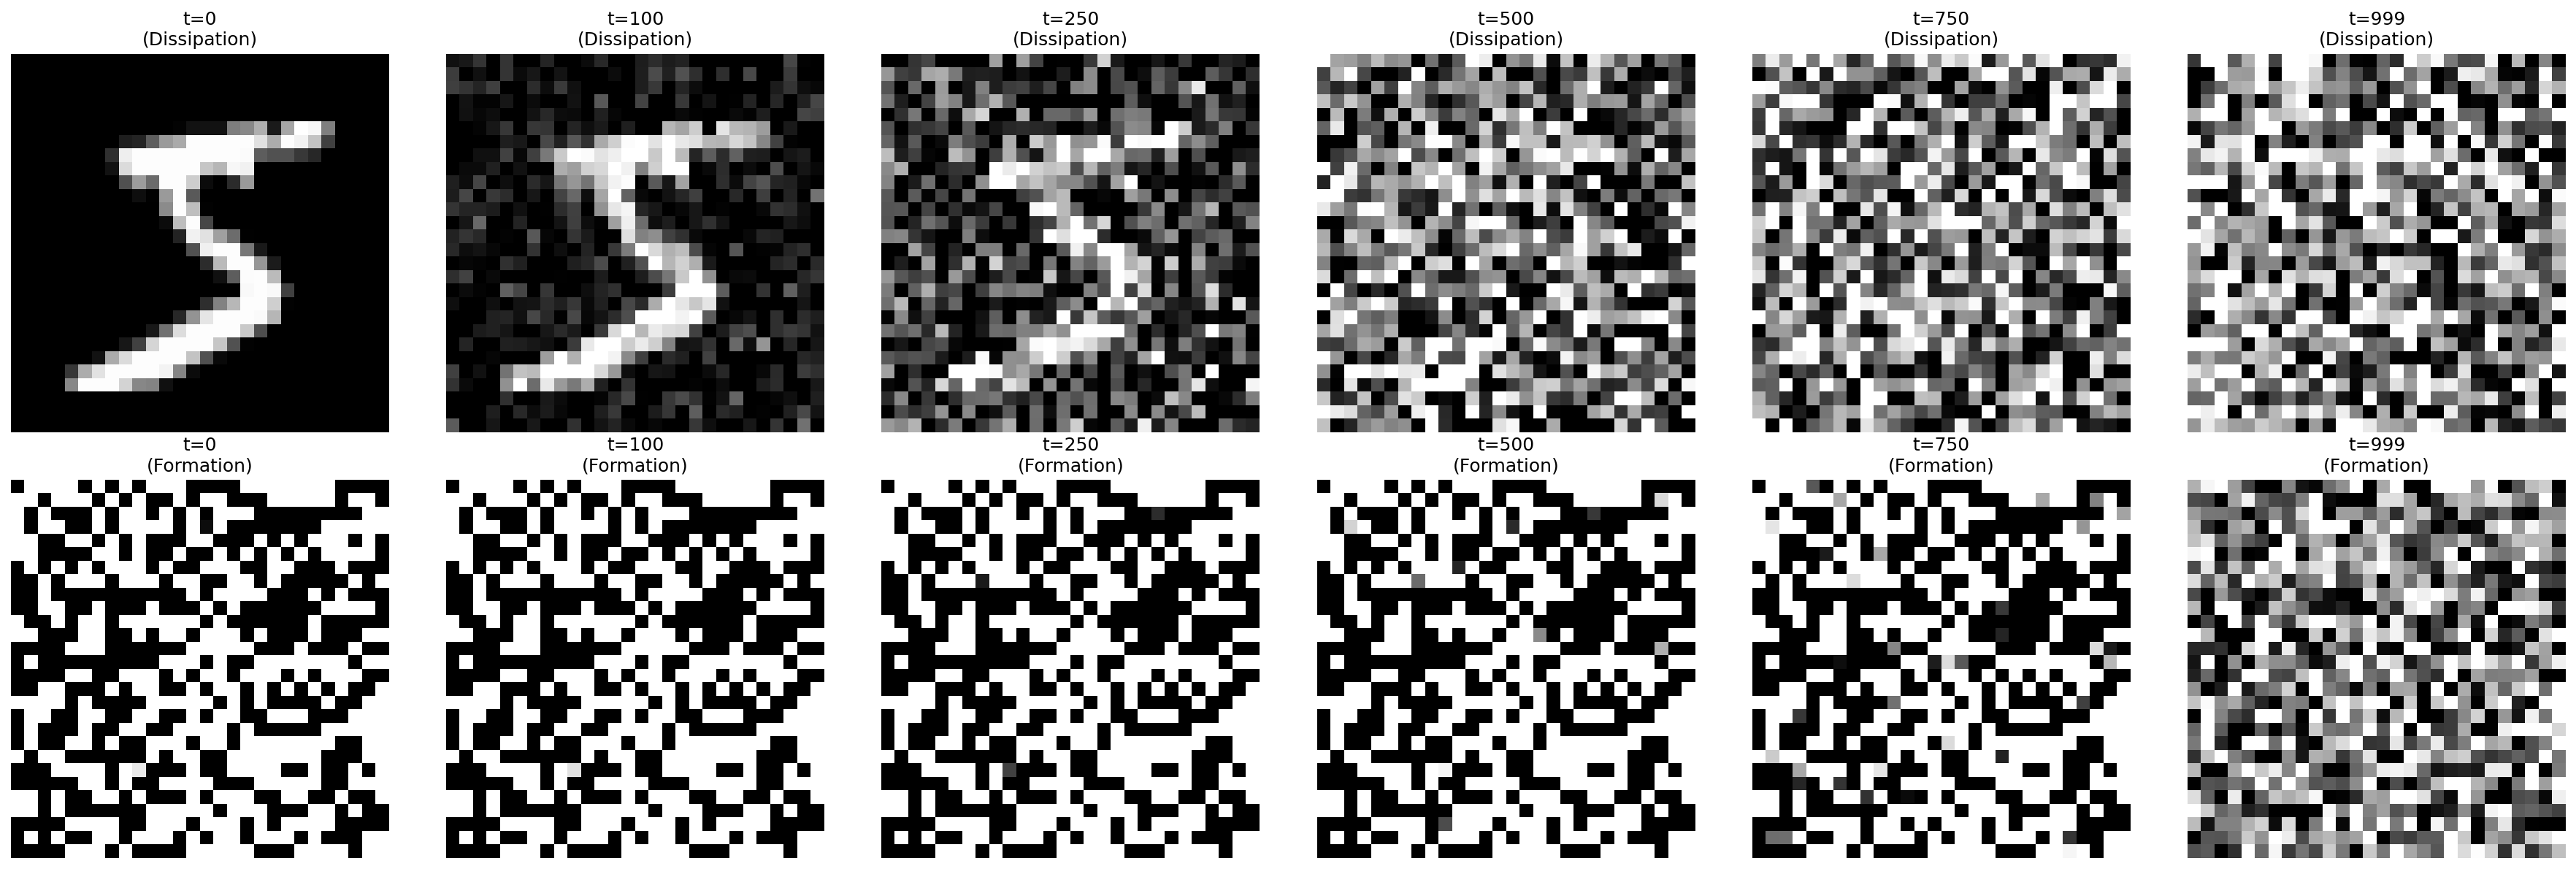
\includegraphics[width=0.8\textwidth]{outputs/trajectories/full_trajectory.png}
    \caption{Full dissipation-formation trajectory. Forward process (left): digit relaxes toward equilibrium. Reverse process (right): structure forms from Gaussian noise.}
    \label{fig:trajectory}
\end{figure}

Training converged to loss $\approx 1.00$ after 30 epochs on CUDA GPU (Titan RTX, 24GB VRAM). Initial loss was 1.507 at epoch 1, decreasing to 1.000642 by epoch 30, demonstrating stable convergence of the learned entropy gradient.

\subsection{Dissipation Schedule Comparison}

We investigated the effect of dissipation schedule choice on trajectory quality. The standard linear schedule $\beta_t = \beta_{\min} + \frac{t}{T}(\beta_{\max} - \beta_{\min})$ was compared against a cosine annealing schedule:

\begin{equation}
\beta_t = \beta_{\min} + \frac{1}{2}(\beta_{\max} - \beta_{\min})\left(1 + \cos\left(\frac{\pi t}{T}\right)\right)
\end{equation}

\begin{figure}[h]
    \centering
    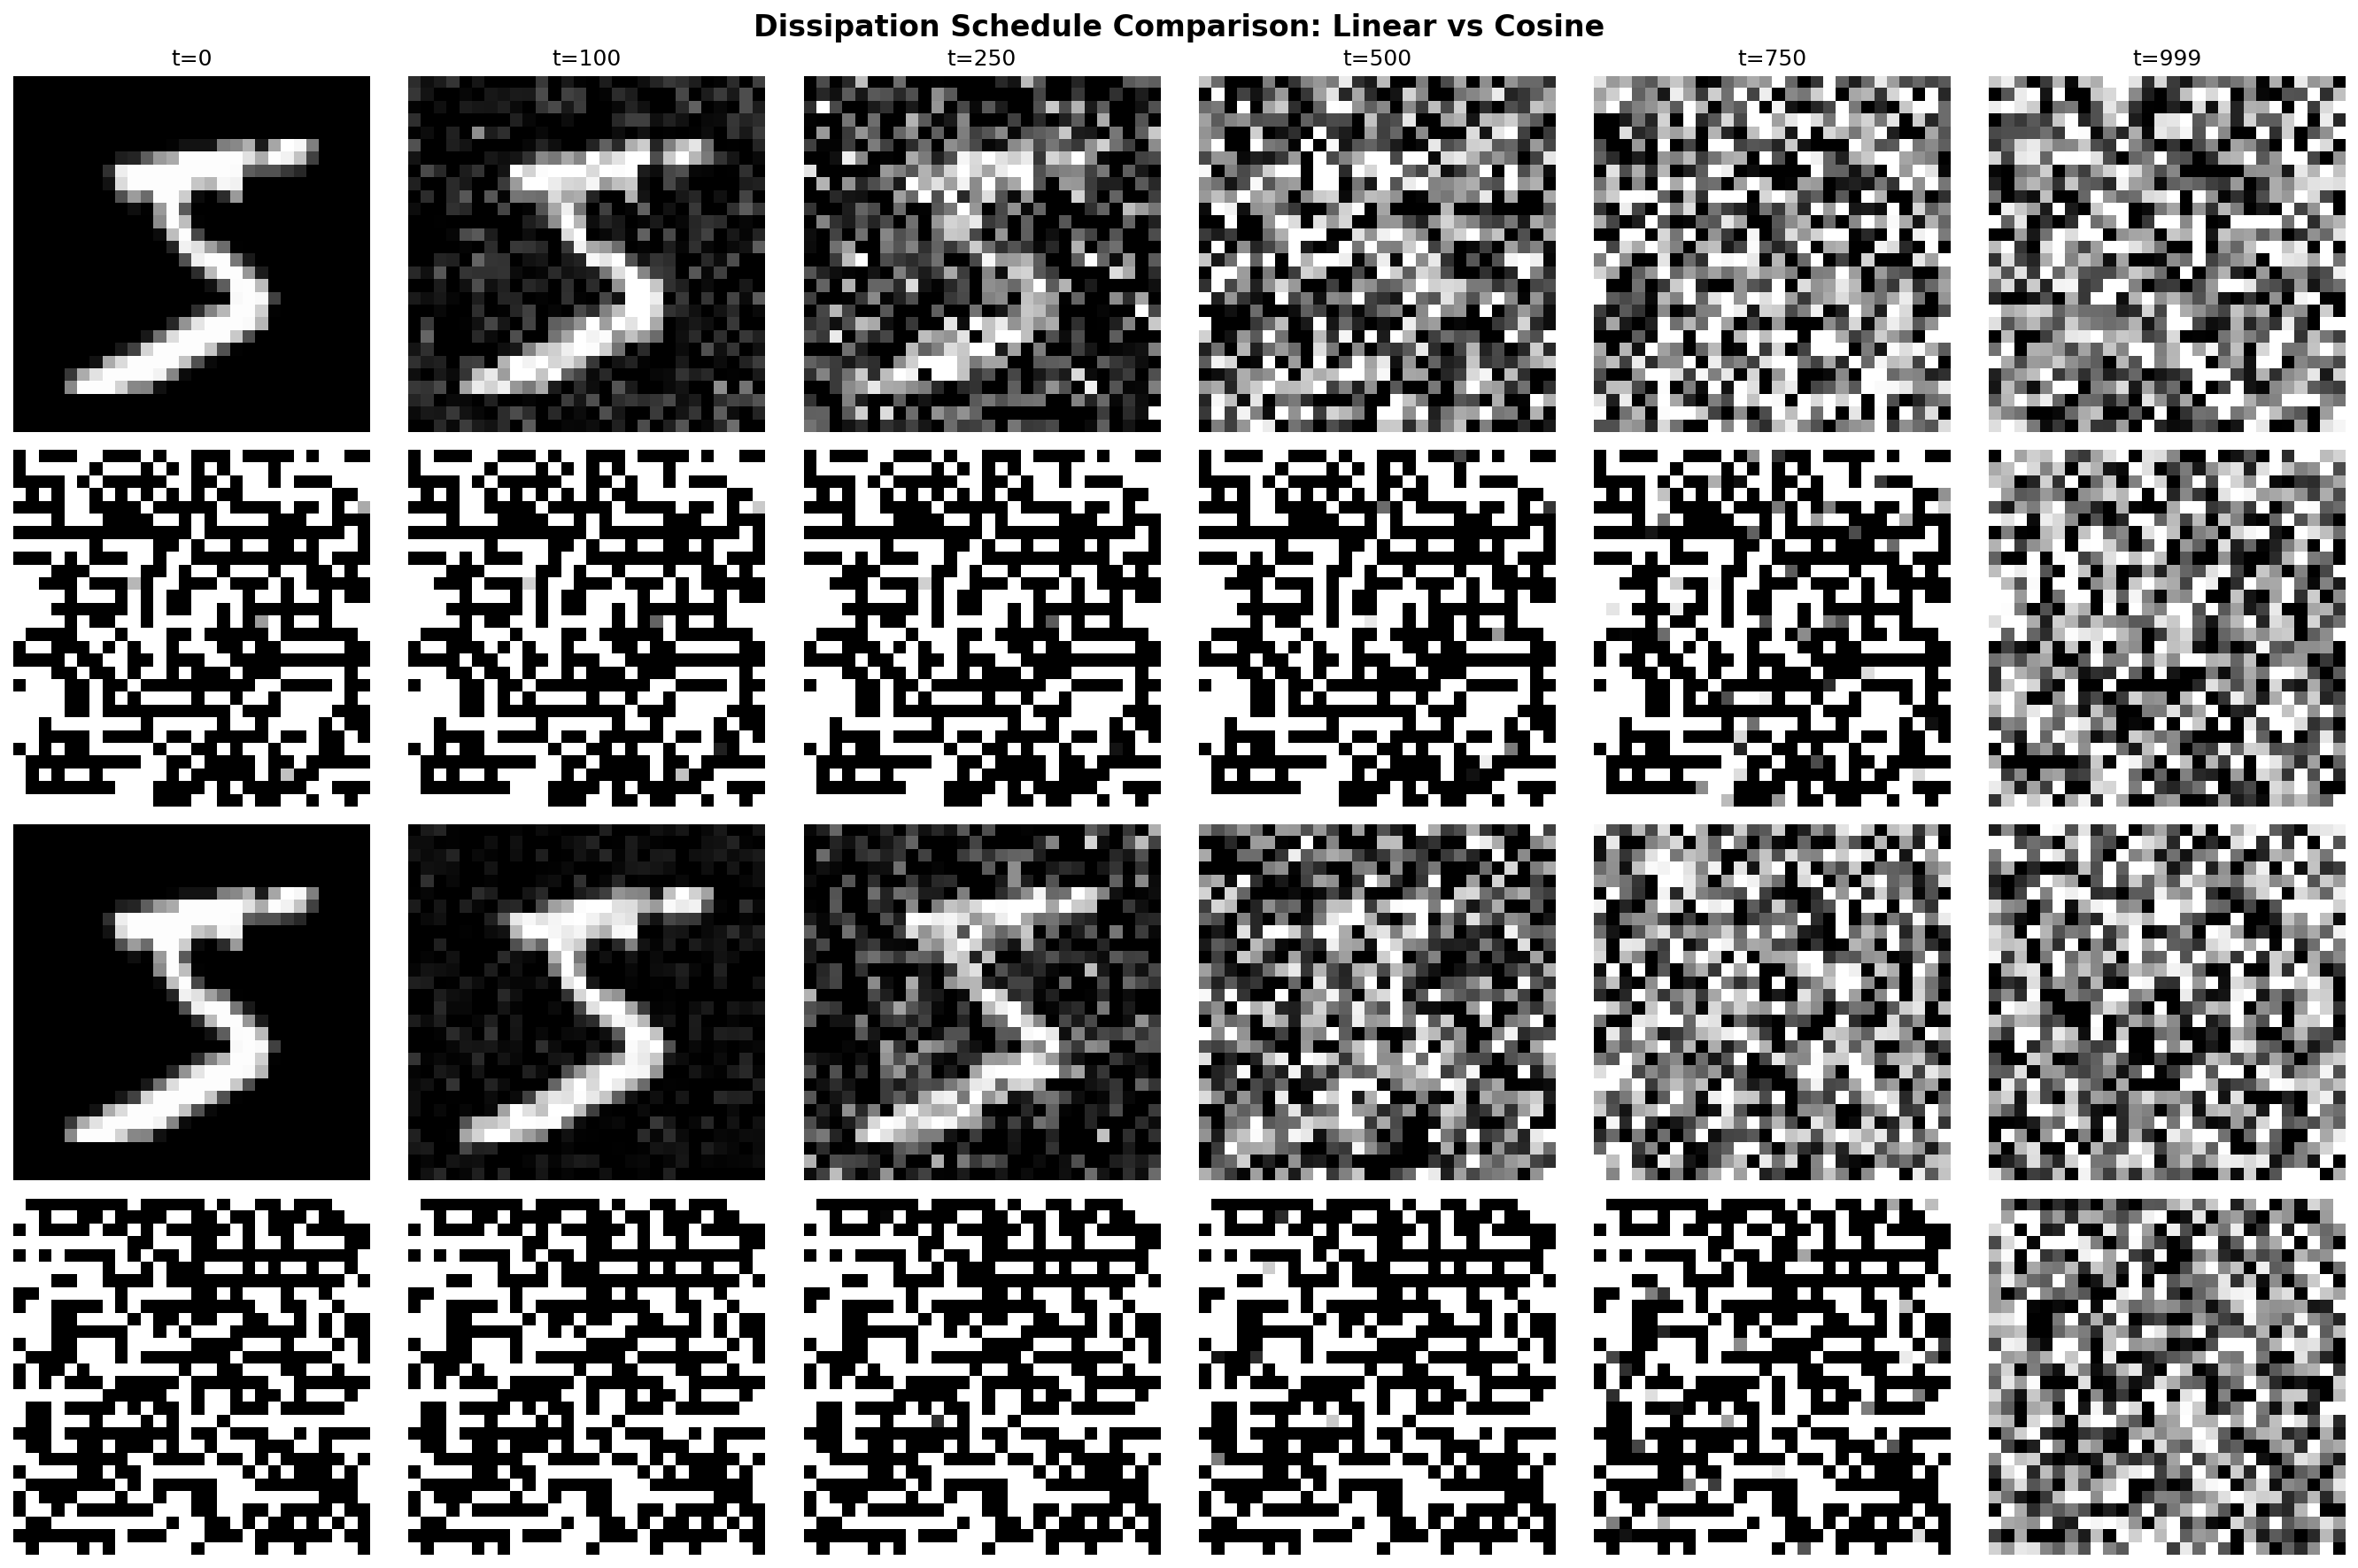
\includegraphics[width=0.9\textwidth]{outputs/trajectories/schedule_comparison.png}
    \caption{Schedule comparison: linear (top two rows) vs cosine (bottom two rows). Forward trajectories show dissipation toward equilibrium; reverse trajectories show formation from noise. Both schedules produce comparable trajectory quality with the same trained constraint field.}
    \label{fig:schedule_comparison}
\end{figure}

The cosine schedule provides smoother entropy injection at trajectory boundaries, potentially improving sample quality in high-dimensional settings. For MNIST, both schedules yield similar formation quality, confirming the robustness of the thermodynamic substrate to schedule parameterisation.

\subsection{Animated Trajectories}

An animated trajectory visualization (Figure \ref{fig:animation}) demonstrates the continuous dissipation-formation process across all 1000 timesteps. The forward process shows gradual relaxation toward maximum entropy, while the reverse process reveals structure emerging via learned energy-gradient traversal.

\begin{figure}[h]
    \centering
    \includegraphics[width=0.6\textwidth]{outputs/trajectories/trajectory_animation.gif}
    \caption{Animated trajectory showing full dissipation-formation cycle. Top: forward process (dissipation). Bottom: reverse process (formation).}
    \label{fig:animation}
\end{figure}

\section{Conclusion}

This implementation demonstrates that diffusion models are not merely "ML architectures" but are \textbf{thermodynamic systems} operating on learned energy landscapes. The forward process is relaxation; the reverse process is formation. The mathematics is the argument.

\section{References}

\begin{itemize}
    \item Sohl-Dickstein et al. (2015). \textit{Deep Unsupervised Learning using Nonequilibrium Thermodynamics.} ICML.
    \item Ho, Jain, \& Abbeel (2020). \textit{Denoising Diffusion Probabilistic Models.} NeurIPS.
    \item Song \& Ermon (2019). \textit{Generative Modeling by Estimating Gradients of the Data Distribution.} NeurIPS.
\end{itemize}

\end{document}
